\documentclass[8pt,aspectratio=169]{beamer}
\usetheme{Madrid}
\usepackage{graphicx}
\usepackage{booktabs}
\usepackage{adjustbox}
\usepackage{multicol}
\usepackage{amsmath}
\usepackage{amssymb}
\usepackage{tikz}
\usepackage{hyperref}
\usepackage{algorithm}
\usepackage{algorithmic}
\usepackage{colortbl}
\usepackage{pgfplots}
\pgfplotsset{compat=1.18}

% TikZ libraries for comics, diagrams, stakeholder maps
\usetikzlibrary{arrows.meta,positioning,shapes.callouts,shapes.geometric,decorations.pathreplacing}

% Color definitions
\definecolor{mlblue}{RGB}{0,102,204}
\definecolor{mlpurple}{RGB}{51,51,178}
\definecolor{mllavender}{RGB}{173,173,224}
\definecolor{mllavender2}{RGB}{193,193,232}
\definecolor{mllavender3}{RGB}{204,204,235}
\definecolor{mllavender4}{RGB}{214,214,239}
\definecolor{mlorange}{RGB}{255, 127, 14}
\definecolor{mlgreen}{RGB}{44, 160, 44}
\definecolor{mlred}{RGB}{214, 39, 40}
\definecolor{mlgray}{RGB}{127, 127, 127}
\definecolor{lightgray}{RGB}{240, 240, 240}
\definecolor{midgray}{RGB}{180, 180, 180}

% NEW COLORS for mini-lecture
\definecolor{dfteal}{RGB}{0,128,128}
\definecolor{dfred}{RGB}{180,30,30}

% Backward compatibility
\colorlet{MLPurple}{mlpurple}
\colorlet{MLBlue}{mlblue}
\colorlet{MLOrange}{mlorange}
\colorlet{MLGreen}{mlgreen}
\colorlet{MLRed}{mlred}
\colorlet{MLLavender}{mllavender}
\colorlet{MLGray}{mlgray}

% Theme colors (exact Madrid settings)
\setbeamercolor{palette primary}{bg=mllavender3,fg=mlpurple}
\setbeamercolor{palette secondary}{bg=mllavender2,fg=mlpurple}
\setbeamercolor{palette tertiary}{bg=mllavender,fg=white}
\setbeamercolor{palette quaternary}{bg=mlpurple,fg=white}
\setbeamercolor{structure}{fg=mlpurple}
\setbeamercolor{section in toc}{fg=mlpurple}
\setbeamercolor{subsection in toc}{fg=mlblue}
\setbeamercolor{title}{fg=mlpurple}
\setbeamercolor{frametitle}{fg=mlpurple,bg=mllavender3}
\setbeamercolor{block title}{bg=mllavender2,fg=mlpurple}
\setbeamercolor{block body}{bg=mllavender4,fg=black}
\setbeamertemplate{navigation symbols}{}
\setbeamertemplate{itemize items}[circle]
\setbeamertemplate{enumerate items}[default]
\setbeamersize{text margin left=5mm,text margin right=5mm}

% Footer
\setbeamertemplate{footline}{
  \leavevmode%
  \hbox{%
    \begin{beamercolorbox}[wd=.333333\paperwidth,ht=2.25ex,dp=1ex,center]{author in head/foot}%
      \usebeamerfont{author in head/foot}Methods and Algorithms
    \end{beamercolorbox}%
    \begin{beamercolorbox}[wd=.333333\paperwidth,ht=2.25ex,dp=1ex,center]{title in head/foot}%
      \usebeamerfont{title in head/foot}MSc Data Science
    \end{beamercolorbox}%
    \begin{beamercolorbox}[wd=.333333\paperwidth,ht=2.25ex,dp=1ex,right]{date in head/foot}%
      \usebeamerfont{date in head/foot}\insertframenumber{} / \inserttotalframenumber\hspace*{2ex}
    \end{beamercolorbox}}%
  \vskip0pt%
}

\newcommand{\bottomnote}[1]{%
\vfill
\vspace{-2mm}
\textcolor{mllavender2}{\rule{\textwidth}{0.4pt}}
\vspace{1mm}
\footnotesize
\textbf{#1}
}

\newenvironment{compactlist}{%
  \begin{itemize}%
    \setlength{\itemsep}{2pt}%
    \setlength{\parskip}{0pt}%
    \setlength{\parsep}{0pt}%
}{%
  \end{itemize}%
}

\newcommand{\highlight}[1]{\textcolor{mlorange}{\textbf{#1}}}
\newcommand{\mathbold}[1]{\boldsymbol{#1}}

\title[KNN Mini-Lecture]{K-Nearest Neighbors}
\subtitle{A 10-Slide Mini-Lecture}
\author{Methods and Algorithms}
\institute{MSc Data Science}
\date{}

\begin{document}

%% ================================================================
%% SLIDE 1: WHY -- TikZ Comic (Dilemma)
%% ================================================================
\begin{frame}[t]{Why Would a Loan Officer Want to Ask the Neighbors?}
\begin{columns}[T]
\column{0.55\textwidth}
\small
\textbf{The Dilemma}
\begin{compactlist}
\item A new applicant walks in with no credit history
\item The rulebook says nothing about this profile
\item But the database holds thousands of past applicants with known outcomes
\end{compactlist}

\vspace{2mm}
What if the answer is already in the data -- hiding among the neighbors?

\begin{block}{Insight}
KNN formalizes human reasoning: when rules fail, look at the most similar past cases and follow their lead.
\end{block}

\column{0.42\textwidth}
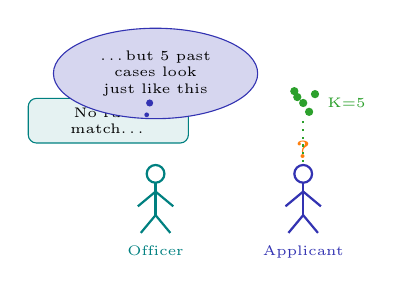
\begin{tikzpicture}[scale=0.75]
% Officer stick figure
\draw[dfteal, thick] (1,2.1) circle (0.15);
\draw[dfteal, thick] (1,1.95) -- (1,1.4);
\draw[dfteal, thick] (1,1.8) -- (0.7,1.55);
\draw[dfteal, thick] (1,1.8) -- (1.3,1.55);
\draw[dfteal, thick] (1,1.4) -- (0.75,1.1);
\draw[dfteal, thick] (1,1.4) -- (1.25,1.1);
\node[dfteal, below, font=\tiny] at (1,1.05) {Officer};
% Applicant stick figure
\draw[mlpurple, thick] (3.5,2.1) circle (0.15);
\draw[mlpurple, thick] (3.5,1.95) -- (3.5,1.4);
\draw[mlpurple, thick] (3.5,1.8) -- (3.2,1.55);
\draw[mlpurple, thick] (3.5,1.8) -- (3.8,1.55);
\draw[mlpurple, thick] (3.5,1.4) -- (3.25,1.1);
\draw[mlpurple, thick] (3.5,1.4) -- (3.75,1.1);
\node[mlpurple, below, font=\tiny] at (3.5,1.05) {Applicant};
\node[mlorange, font=\small\bfseries] at (3.5,2.5) {?};
% Speech bubble
\node[draw=dfteal, fill=dfteal!10, rounded corners=3pt,
      font=\tiny, text width=1.8cm, align=center]
      at (0.2,3.0) {No rules match\ldots};
% Thought bubble
\node[draw=mlpurple, fill=mllavender4, ellipse,
      font=\tiny, text width=1.6cm, align=center]
      at (1.0,3.8) {\ldots but 5 past cases look just like this};
\fill[mlpurple] (0.85,3.1) circle (0.04);
\fill[mlpurple] (0.9,3.3) circle (0.06);
% Neighbor cluster
\foreach \dx/\dy in {0/0, 0.2/0.15, -0.15/0.2, 0.1/-0.15, -0.1/0.1} {
  \fill[mlgreen] (3.5+\dx, 3.3+\dy) circle (0.07);
}
\draw[dotted, mlgreen, thick] (3.5,2.3) -- (3.5,3.0);
\node[mlgreen, font=\tiny, right] at (3.75,3.3) {K=5};
\end{tikzpicture}
\end{columns}

\bottomnote{Instance-based learning stores all training data -- no model parameters, no training phase}
\end{frame}

%% ================================================================
%% SLIDE 2: FEEL -- Text-Only with Prompt
%% ================================================================
\begin{frame}[t]{Classifying a Stranger -- Did Similarity Cross Your Mind?}
\begin{columns}[T]
\column{0.55\textwidth}
\small
\textbf{Think Before You Compute}

\footnotesize
Imagine you meet someone at a conference. You know nothing about them. Within seconds, your brain classifies: academic or industry? Junior or senior? You did not run a logistic regression. You compared them to people you already know.

\begin{compactlist}
\item How many ``neighbors'' did your brain consult?
\item Did you weight closer acquaintances more heavily?
\item What ``features'' did you use -- appearance, speech, context?
\end{compactlist}

\begin{exampleblock}{Reflection Prompt}
Write down one real decision you made this week by mentally consulting similar past cases. What K did you use?
\end{exampleblock}

\column{0.42\textwidth}
\footnotesize
\vspace{4mm}
\fcolorbox{mlpurple}{mllavender4}{\parbox{0.85\columnwidth}{%
\textbf{Pause and reflect:}

\vspace{2mm}
When you last recommended a restaurant to a friend, did you match their taste to similar friends who liked similar places?

\vspace{2mm}
\textbf{That is KNN.}
}}
\end{columns}

\bottomnote{KNN mirrors how humans naturally classify: by analogy to known examples, not by learned rules}
\end{frame}

%% ================================================================
%% SLIDE 3: WHAT -- Comparison Table
%% ================================================================
\begin{frame}[t]{What Makes KNN Different from Logistic Regression and Trees?}
\begin{columns}[T]
\column{0.55\textwidth}
\small
\textbf{Taxonomy of Classifiers}

\vspace{1mm}
\footnotesize
\begin{tabular}{@{}l c c c@{}}
\toprule
\textbf{Property} & \textbf{\textcolor{dfteal}{KNN}} & \textbf{Log.\ Reg.} & \textbf{Dec.\ Tree} \\
\midrule
\rowcolor{mllavender4}
Training & None & Optimize & Build tree \\
Boundary & Local & Linear & Axis-aligned \\
\rowcolor{mllavender4}
Interpret. & Low & High & High \\
New classes & Natural & Retrain & Retrain \\
\rowcolor{mllavender4}
Memory & All data & Params & Tree only \\
Speed & O(nd) & O(d) & O(depth) \\
\bottomrule
\end{tabular}

\vspace{2mm}
\scriptsize\textbf{Pattern:} KNN trades training speed for prediction cost -- the opposite of parametric models.

\begin{block}{Insight}
\scriptsize Lazy learners memorize; eager learners generalize. KNN defers all computation to prediction time.
\end{block}

\column{0.42\textwidth}
\footnotesize
\vspace{2mm}
\colorbox{dfteal!15}{\parbox{0.9\columnwidth}{\textbf{KNN:} Lazy, local, non-parametric}}

\vspace{3mm}
\colorbox{mlorange!15}{\parbox{0.9\columnwidth}{\textbf{LogReg:} Eager, global, parametric}}

\vspace{3mm}
\colorbox{mlpurple!15}{\parbox{0.9\columnwidth}{\textbf{Tree:} Eager, local, non-parametric}}
\end{columns}

\bottomnote{Non-parametric means the model complexity grows with the data -- no fixed number of parameters}
\end{frame}

%% ================================================================
%% SLIDE 4: CASE -- Step Diagram / Timeline
%% ================================================================
\begin{frame}[t]{What Happens When One Applicant Enters the Feature Space?}
\begin{columns}[T]
\column{0.55\textwidth}
\small
\textbf{One Prediction, Step by Step}
\begin{compactlist}
\item Applicant arrives with feature vector (income, debt ratio, employment length)
\item All features standardized to zero mean, unit variance
\item Algorithm computes distance to every stored example
\item K closest examples ``vote'' on the label
\item Majority wins; ties broken by distance weighting
\end{compactlist}

\begin{block}{Insight}
\scriptsize Feature standardization is not optional -- without it, high-magnitude features dominate the distance.
\end{block}

\column{0.42\textwidth}
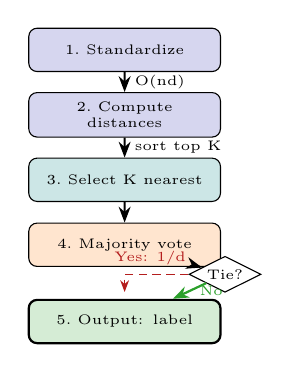
\begin{tikzpicture}[scale=0.75,
  stepnode/.style={draw, rounded corners=3pt, font=\tiny,
    text width=2.2cm, align=center, minimum height=0.55cm},
  arr/.style={-{Stealth[length=2mm]}, thick}]
% Nodes
\node[stepnode, fill=mllavender4] (s1) at (1.5,5.0) {1.\ Standardize};
\node[stepnode, fill=mllavender4] (s2) at (1.5,3.9) {2.\ Compute distances};
\node[stepnode, fill=dfteal!20]   (s3) at (1.5,2.8) {3.\ Select K nearest};
\node[stepnode, fill=mlorange!20] (s4) at (1.5,1.7) {4.\ Majority vote};
\node[stepnode, fill=mlgreen!20, thick] (s5) at (1.5,0.4) {5.\ Output: label};
% Arrows with labels
\draw[arr] (s1) -- (s2) node[midway, right, font=\tiny] {O(nd)};
\draw[arr] (s2) -- (s3) node[midway, right, font=\tiny] {sort top K};
\draw[arr] (s3) -- (s4);
% Decision diamond
\node[draw, diamond, fill=white, font=\tiny,
      inner sep=1pt, aspect=2] (tie) at (3.2,1.2) {Tie?};
\draw[arr] (s4) -- (tie);
\draw[arr, mlgreen] (tie) -- (s5) node[midway, right, font=\tiny] {No};
\draw[-{Stealth[length=1.5mm]}, dfred, densely dashed]
  (tie.west) -| (1.5,0.9) node[pos=0.3, above, font=\tiny] {Yes: 1/d};
\end{tikzpicture}
\end{columns}

\bottomnote{Complexity per query: O(nd) for brute force, O(n log n) with KD-trees when d is small}
\end{frame}

%% ================================================================
%% SLIDE 5: HOW -- Side-by-Side Architecture
%% ================================================================
\begin{frame}[t]{Who Should Measure Distance -- Euclid, Manhattan, or Cosine?}
\begin{columns}[T]
\column{0.55\textwidth}
\small
\textbf{Three Distance Philosophies}
\begin{compactlist}
\item \textbf{Euclidean} (L2): straight-line, default for dense numerical data
\item \textbf{Manhattan} (L1): city-block, robust to outliers
\item \textbf{Cosine}: measures angle not magnitude, ideal for sparse high-D
\end{compactlist}

\vspace{1mm}
\scriptsize The choice of metric reshapes which points count as neighbors.

\begin{block}{Insight}
\scriptsize Euclidean assumes all features equally scaled and important. When that fails, Manhattan or Cosine often outperform.
\end{block}

\column{0.42\textwidth}
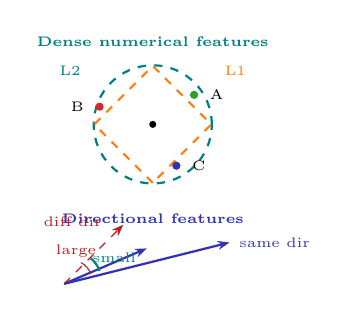
\begin{tikzpicture}[scale=0.75]
% -- Top: Euclidean circle vs Manhattan diamond --
\node[font=\tiny\bfseries, dfteal] at (1.5,4.6) {Dense numerical features};
\fill[black] (1.5,3.2) circle (0.06);
\draw[dfteal, dashed, thick] (1.5,3.2) circle (1.0);
\draw[mlorange, dashed, thick, rotate around={45:(1.5,3.2)}]
  (0.8,2.5) rectangle (2.2,3.9);
% Data points
\fill[mlgreen] (2.2,3.7) circle (0.07);
\node[font=\tiny, right] at (2.3,3.7) {A};
\fill[mlred] (0.6,3.5) circle (0.07);
\node[font=\tiny, left] at (0.5,3.5) {B};
\fill[mlpurple] (1.9,2.5) circle (0.07);
\node[font=\tiny, right] at (2.0,2.5) {C};
\node[font=\tiny, dfteal] at (0.1,4.1) {L2};
\node[font=\tiny, mlorange] at (2.9,4.1) {L1};
% -- Bottom: Cosine --
\node[font=\tiny\bfseries, mlpurple] at (1.5,1.6) {Directional features};
\draw[-{Stealth[length=1.5mm]}, mlpurple, thick]
  (0,0.5) -- (2.8,1.2);
\draw[-{Stealth[length=1.5mm]}, mlpurple, thick]
  (0,0.5) -- (1.4,1.1);
\draw[-{Stealth[length=1.5mm]}, dfred, dashed]
  (0,0.5) -- (1.0,1.5);
\draw[dfteal, thick] (0.6,0.72) arc (20:50:0.5);
\node[font=\tiny, dfteal] at (0.85,0.95) {small};
\draw[dfred] (0.45,0.67) arc (20:62:0.35);
\node[font=\tiny, dfred] at (0.2,1.05) {large};
\node[font=\tiny, mlpurple, right] at (2.8,1.2) {same dir};
\node[font=\tiny, dfred, left] at (0.8,1.55) {diff dir};
\end{tikzpicture}
\end{columns}

\bottomnote{Also consider: Mahalanobis (correlated features), Hamming (binary features)}
\end{frame}

%% ================================================================
%% SLIDE 6: RISK -- TikZ Comic (Failure Scene)
%% ================================================================
\begin{frame}[t]{What Could Go Wrong If Every Dimension Votes Equally?}
\begin{columns}[T]
\column{0.55\textwidth}
\small
\textbf{Three Ways KNN Fails Silently}
\begin{compactlist}
\item \textbf{Curse of dimensionality}: in high-D, all points become equidistant
\item \textbf{Wrong K}: too small = noise, too large = local structure lost
\item \textbf{Imbalanced classes}: majority dominates the vote
\end{compactlist}

\begin{block}{Insight}
\scriptsize The curse of dimensionality is not theoretical trivia -- adding irrelevant features silently degrades KNN.
\end{block}

\column{0.42\textwidth}
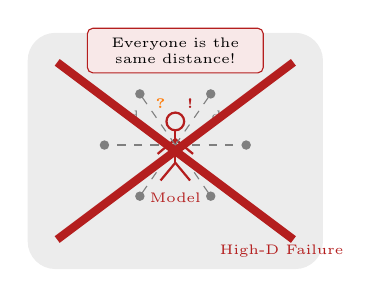
\begin{tikzpicture}[scale=0.75]
% Fog background
\fill[mlgray!15, rounded corners=10pt] (0,0) rectangle (5,4);
% Model stick figure in center
\draw[dfred, thick] (2.5,2.5) circle (0.15);
\draw[dfred, thick] (2.5,2.35) -- (2.5,1.8);
\draw[dfred, thick] (2.5,2.2) -- (2.2,1.95);
\draw[dfred, thick] (2.5,2.2) -- (2.8,1.95);
\draw[dfred, thick] (2.5,1.8) -- (2.25,1.5);
\draw[dfred, thick] (2.5,1.8) -- (2.75,1.5);
\node[dfred, below, font=\tiny] at (2.5,1.45) {Model};
\node[mlorange, font=\tiny\bfseries] at (2.25,2.8) {?};
\node[dfred, font=\tiny\bfseries] at (2.75,2.8) {!};
% 6 equidistant data points (0,60,120,180,240,300 deg)
\foreach \angle in {0,60,120,180,240,300} {
  \fill[mlgray] ({2.5+1.2*cos(\angle)}, {2.1+1.0*sin(\angle)}) circle (0.08);
  \draw[mlgray, dashed] (2.5,2.1) -- ({2.5+1.2*cos(\angle)}, {2.1+1.0*sin(\angle)});
}
\node[font=\tiny, mlgray] at (3.2,2.6) {d};
\node[font=\tiny, mlgray] at (1.8,2.6) {d};
% Speech bubble
\node[draw=dfred, fill=dfred!10, rounded corners=2pt,
      font=\tiny, text width=2.0cm, align=center]
      at (2.5,3.7) {Everyone is the same distance!};
% Large X
\draw[dfred, line width=3pt] (0.5,0.5) -- (4.5,3.5);
\draw[dfred, line width=3pt] (0.5,3.5) -- (4.5,0.5);
\node[font=\tiny, dfred] at (4.3,0.3) {High-D Failure};
\end{tikzpicture}
\end{columns}

\bottomnote{Mitigation: feature selection, PCA for dimensionality reduction, distance-weighted voting}
\end{frame}

%% ================================================================
%% SLIDE 7: WHERE -- Chart (External PDF)
%% ================================================================
\begin{frame}[t]{Why Do So Many Practitioners Start with KNN?}
\begin{columns}[T]
\column{0.55\textwidth}
\small
\textbf{KNN as a Baseline Classifier}
\begin{compactlist}
\item No assumptions about data distribution
\item Naturally handles multi-class problems
\item Decision boundaries adapt to local density
\item Fast to prototype: only K to tune
\end{compactlist}

\vspace{1mm}
\scriptsize The chart shows how boundaries smooth as K increases.

\begin{block}{Insight}
\scriptsize KNN decision boundaries emerge from the data, not from optimization. This makes KNN the natural first-look tool.
\end{block}

\column{0.42\textwidth}
\vspace{2mm}
\includegraphics[width=\textwidth]{01_knn_boundaries/chart.pdf}
\end{columns}

\bottomnote{KNN with K=1 achieves asymptotic error at most twice Bayes optimal (Cover--Hart theorem)}
\end{frame}

%% ================================================================
%% SLIDE 8: IMPACT -- Stakeholder Map
%% ================================================================
\begin{frame}[t]{Who Wins and Who Loses When KNN Replaces Rules?}
\begin{columns}[T]
\column{0.55\textwidth}
\small
\textbf{Stakeholder Analysis}
\begin{compactlist}
\item \textbf{Winners}: Risk teams, medical teams, marketing (segmentation)
\item \textbf{Losers}: Compliance (hard to explain), IT ops (latency scales with data)
\end{compactlist}

\vspace{1mm}
\scriptsize KNN shifts power from those who write rules to those who curate data.

\begin{block}{Insight}
\scriptsize KNN's Achilles heel in regulated industries is not accuracy -- it is explainability.
\end{block}

\column{0.42\textwidth}
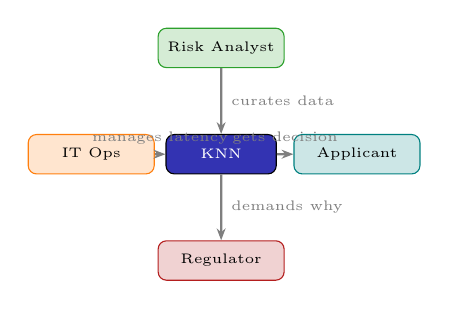
\begin{tikzpicture}[scale=0.75,
  actor/.style={draw, rounded corners=3pt, font=\tiny,
    minimum width=1.6cm, minimum height=0.5cm, align=center},
  arr/.style={-{Stealth[length=1.5mm]}, thick, mlgray}]
% Center
\node[actor, fill=mlpurple, text=white, minimum width=1.4cm] (knn) at (2.2,2.2) {KNN};
% Top: Risk Analyst
\node[actor, fill=mlgreen!20, draw=mlgreen] (risk) at (2.2,4.0) {Risk Analyst};
\draw[arr] (risk) -- (knn) node[midway, right, font=\tiny] {curates data};
% Right: Applicant
\node[actor, fill=dfteal!20, draw=dfteal] (app) at (4.5,2.2) {Applicant};
\draw[arr] (knn) -- (app) node[midway, above, font=\tiny] {gets decision};
% Bottom: Regulator
\node[actor, fill=dfred!20, draw=dfred] (reg) at (2.2,0.4) {Regulator};
\draw[arr] (knn) -- (reg) node[midway, right, font=\tiny] {demands why};
% Left: IT Ops
\node[actor, fill=mlorange!20, draw=mlorange] (it) at (0,2.2) {IT Ops};
\draw[arr] (it) -- (knn) node[midway, above, font=\tiny] {manages latency};
\end{tikzpicture}
\end{columns}

\bottomnote{Explainability: show the K neighbors and their features as the reason for classification}
\end{frame}

%% ================================================================
%% SLIDE 9: SO WHAT -- Balance Scale
%% ================================================================
\begin{frame}[t]{3 Questions That Reveal Whether KNN Is the Right Algorithm}
\begin{columns}[T]
\column{0.55\textwidth}
\small
\textbf{The Decision Framework}
\begin{enumerate}
\setlength{\itemsep}{2pt}
\item \textbf{Is the data low-dimensional?} -- If d $>$ 20, distances lose meaning
\item \textbf{Is the training set storable?} -- If n $>$ 1M, consider approximate methods
\item \textbf{Can you live without a formula?} -- If regulators demand one, look elsewhere
\end{enumerate}

\vspace{1mm}
\scriptsize If all three answers are yes, KNN is a strong candidate.

\begin{block}{Insight}
\scriptsize No algorithm is universally best. KNN excels in low dimensions, moderate data, local patterns.
\end{block}

\column{0.42\textwidth}
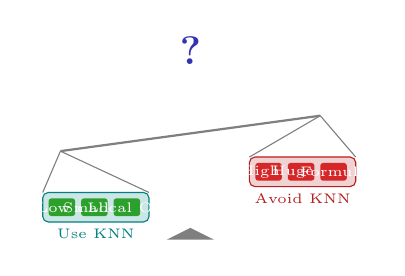
\begin{tikzpicture}[scale=0.75]
% Fulcrum
\fill[mlgray] (2.5,0.2) -- (2.1,0) -- (2.9,0) -- cycle;
% Beam (tilted: left lower = KNN wins)
\draw[thick, mlgray] (0.3,1.5) -- (4.7,2.1);
% Left pan: Use KNN
\draw[mlgray] (0.3,1.5) -- (0.0,0.8);
\draw[mlgray] (0.3,1.5) -- (1.8,0.8);
\draw[dfteal, fill=dfteal!20, rounded corners=2pt]
  (0.0,0.3) rectangle (1.8,0.8);
\foreach \i/\txt in {0/Low d, 1/Small n, 2/Local OK} {
  \fill[mlgreen, rounded corners=1pt]
    (0.1+\i*0.55, 0.4) rectangle (0.55+\i*0.55, 0.7);
  \node[font=\tiny, white] at (0.33+\i*0.55, 0.55) {\txt};
}
\node[font=\tiny, dfteal] at (0.9,0.1) {Use KNN};
% Right pan: Avoid KNN
\draw[mlgray] (4.7,2.1) -- (3.5,1.4);
\draw[mlgray] (4.7,2.1) -- (5.3,1.4);
\draw[dfred, fill=dfred!20, rounded corners=2pt]
  (3.5,0.9) rectangle (5.3,1.4);
\foreach \i/\txt in {0/High d, 1/Huge n, 2/Formula} {
  \fill[mlred, rounded corners=1pt]
    (3.6+\i*0.55, 1.0) rectangle (4.05+\i*0.55, 1.3);
  \node[font=\tiny, white] at (3.83+\i*0.55, 1.15) {\txt};
}
\node[font=\tiny, dfred] at (4.4,0.7) {Avoid KNN};
% Question mark
\node[mlpurple, font=\Large\bfseries] at (2.5,3.2) {?};
\end{tikzpicture}
\end{columns}

\bottomnote{The No Free Lunch theorem guarantees no single algorithm dominates across all datasets}
\end{frame}

%% ================================================================
%% SLIDE 10: ACT -- Activity Frame
%% ================================================================
\begin{frame}[t]{Can You Evaluate This Real Classification Problem?}
\begin{columns}[T]
\column{0.55\textwidth}
\small
\textbf{The Scenario}

\footnotesize
A retail bank wants to predict loan defaults. Features: income, age, employment length, debt-to-income, number of open accounts. The dataset has moderate size and all features are numerical.

\begin{compactlist}
\item Apply the 3-question framework from the previous slide
\item Decide: Is KNN appropriate here?
\item If yes: recommend K and distance metric
\item If no: name a better algorithm
\end{compactlist}

\begin{exampleblock}{Deliverable}
\scriptsize Fill in the table. Be prepared to defend your verdict to a skeptical risk manager.
\end{exampleblock}

\column{0.42\textwidth}
\footnotesize
\vspace{2mm}
\begin{tabular}{@{}l p{2.8cm}@{}}
\toprule
\textbf{Question} & \textbf{Your Answer} \\
\midrule
Low-dimensional? & \rule{2.5cm}{0.4pt} \\[3pt]
Storable data? & \rule{2.5cm}{0.4pt} \\[3pt]
Example-based OK? & \rule{2.5cm}{0.4pt} \\[3pt]
\textbf{Verdict} & \rule{2.5cm}{0.4pt} \\[3pt]
Recommended K & \rule{2.5cm}{0.4pt} \\[3pt]
Distance metric & \rule{2.5cm}{0.4pt} \\
\bottomrule
\end{tabular}
\end{columns}

\bottomnote{Hint: consider dimensionality, data size, and regulatory environment}
\end{frame}

\end{document}
